\chapter{Smartphones as Population Density Trackers}
\label{chap:lit-review}
Modern smartphones provide unparalleled opportunities for people to access ever innovating services. This in turn creates a volatility that makes the mobile landscape of the future difficult to predict and many are unsure what form it will take in even the near future. This chapter aims to provide an understanding of this industrial landscape and outline the demand and technical description of crowd-sourced mobile applications and their ability to analyse and predict population density.

\section{Smartphone Access and Development}

The rise in competition within the low-priced smartphone market from brands like Huawei and Samsung have created a revolution in South Africa in terms of Internet access. As of 2019, over 91\% of South Africans have access to a smartphone and all the global connectivity that accompanies it \cite{ICASA2020}. This combined with near total 3G network coverage \cite{ICASA2020} means that almost all South Africans have become part of the online smartphone application ecosystem. Cheap data-based communication applications like WhatsApp and Facebook Messenger have largely replaced SMS, and revolutionary services like Uber and UberEats have had a similar effect on the taxicab and food delivery industries. Contemporary smartphone applications have sculpted our way of life and this trend is accelerating as we more closely understand what advancements the smartphone revolution has in store for us.

\subsection{App Development}
Android and iOS app development have never been easier with the release of 1st party toolsets like Android Studio and Xcode which allow anyone with the slightest programming background to start working on their application idea. Access to a global market where the barrier for entry for businesses is low and the potential customer base is in the billions \cite{Turner}, has made smartphone application development a priority for companies wanting access to this \$311.25 billion market \cite{AlliedMarketResearch2019}.

South Africa is no exception to this economic surge with over four thousand apps available on the Google Play Store with nearly 200 million downloads across them \cite{42matters}. Unfortunately, expensive data prices are a major obstacle preventing South Africa from reaching its potential in harnessing the economic benefits of smartphones. South Africa is ranked 148th out of 228 countries in terms of mobile data prices, which may not seem that prohibitive when compared to the United States (188th) and New Zealand (180th) \cite{Cable.co.uk}, but doesn’t take into account the large proportion of the population that can only purchase data in smaller packages. Data when purchased in the 10s of Gigabytes may not be that bad a deal, but South Africa’s large impoverished population are forced to buy data at disproportionately expensive prices due to mobile data’s exploitative pricing structure. 
Despite prohibitive data price-structures, the number of smartphone application downloads is likely to accelerate moving forward, due to the Competition Commission’s order on mobile-service operators to lower their exorbitant data prices. The implementation of this order has created an average price drop of 33\% across all affected data packages \cite{Bottomley2020}. The continued adoption of smartphones and lowered data prices is likely to accelerate South Africa’s application development marketplace into a thriving economic sector in the near future.

\subsection{Smartphone Technology}
A smartphone’s convenience is in a large part due to the considerable number of sensors at its disposal. While the number and types of sensors vary from phone to phone, there are several sensors that are seen as necessary, by the market, for a smartphone to feel complete. 

\begin{table}[]
    \begin{tabular}{lll}
    \hline
    \textbf{Sensor} & \textbf{Function}                                       & \textbf{Prevalence} \\ \hline
    Accelerometer   & Detects acceleration and vibration.                     & High                \\
    Ambient Light   & Determines ambient light levels.                        & High                \\
    Barometer       & Measures air pressure.                                  & Low                 \\
    Bluetooth       & Used for data exchange over short distances.            & High                \\
    Camera          & Used to take optical images.                            & High                \\
    Cellular        & Used to connect to cellular networks.                   & High                \\
    Fingerprint     & Biometric sensor used to verify user’s identity.        & Low                 \\
    GPS             & Determines geographical position.                       & High                \\
    Gyroscope       & Detects Orientation and rotation.                       & High                \\
    Heart Rate      & Detects user’s heart rate.                              & Low                 \\
    Magnetometer    & Detects magnetic fields.                                & High                \\
    Microphone      & Detects and records sound.                              & High                \\
    Proximity       & Uses infrared light to detect proximity to device.      & High                \\
    Thermometer     & Monitors internal temperature.                          & High                \\
    Touchscreen     & Capacitive sensors that detect interaction with screen. & High                \\
    Wi-Fi           & Used to connect to local Wi-Fi hotspots.                & High                \\ \hline
    \end{tabular}
    \caption{: list of sensors found in smartphones and their market prevalence \cite{Priyadarshini2018}.}
    \label{tab:lit_sensors}
\end{table}

Many newer smartphones tend to market themselves either on the fidelity of their sensors, often in the case of cameras, or the existence of a newly added one. An example of companies using newer sensors to sell devices is the iPhone 12 Pro’s incorporation of a LiDAR sensor to be used for more immersive AR experiences \cite{Stein2020}. The sheer number of sensors in smartphones provide developers plenty of opportunities for creative methods of solving problems. This can mean that for determining the smartphone’s location, an application could use a combination of GPS, Cellular, Wi-fi and Bluetooth sensors to create a highly accurate approximation of the user’s current position.

\section{Data Collection}
Our collective overreliance on the use of smartphones have led them to become an extension of our own thoughts and desires. They store our calendars, our shopping lists, our photos, and our private conversations. In this, they also store desirable data for companies to be used in various applications including revenue collection through advertising, and diagnostic data used to improve their own applications. This enticing amalgamation of information has led to an explosive amount of free smartphone apps that use the user’s personal information and telemetric data as payment for their services. This has placed consumers in a predicament where they must choose between their privacy, or anonymity, and the countless number of useful applications which will inevitably raise their standard of living. 

\subsection{Crowd Sourced Data}
The universal nature of smartphones has made them prime conduits for sourcing large amounts of unique data points. Each app download is not only a potential revenue stream for its owner, but also a contributor to a wider network of information. This has led to the rise of crowd-sourced applications which can be found in an abundance on both Android and iOS app-stores.

Crowd-sourcing is defined by Merriam-Webster as “the practice of obtaining needed services, ideas, or content by soliciting contributions from a large group of people”\cite{Merriam-Webster}. This definition indicates that there are a few key criteria that a smartphone App needs to meet for it to be implementing crowdsourcing. Firstly, it must be collecting data that is being used to supply a service to its customers, itself or a third party. Secondly, it must have a large enough install base so that the data gathered is useful. While the first aspect is easy to implement, the success of any crowd sourcing application depends on its ability to accrue a large enough user base for the data gathered to be useful. An App which reviews destinations, for example, is only useful if it has enough user reviews for the App to provide meaningful reviews to its audience. 

An example of a successful crowd-sourcing smartphone application is Zomato, which crowd-sources restaurant reviews and uses them to help customers choose where to eat. With nearly 10 million reviews, Zomato’s large userbase provides both the company and its users with diverse and statistically significant information on where to buy food. The success of this app also demonstrates the cyclic nature of crowdsourcing applications. As you accrue more users, the data that you crowdsource is more useful which incentivises more users to join. However, the contrary is also true, where if you fail to achieve a high enough user base, the information you provide will not be useful enough to sustain your audience and, hence, your audience will shrink indefinitely.

Crowd sourcing Apps are therefore incentivised to gather proxies for their desired information to bolster their database. Smartphones’ diverse set of sensors, detailed in Table 1, provide the option for apps to find non-conventional methods of accruing data. As an example, the crowd-sourced application Pothole Patrol, developed by MIT for monitoring road surfaces, uses a combination of location services and the phones built in vibration sensors to track and report pothole locations \cite{eriksson2008pothole}. While the acceleration data gathered by the vibration sensors would not normally be used for this type of analysis, smartphone sensors provide developers with the ability to solve design decisions in interesting and innovative ways. 

\subsection{Location Tracking Services}
There are two primary mechanisms of determining your location via mobile connection: position-tracking services and position-aware services. Location-tracking services entail using external party’s resources to track and maintain the locational data relevant to the user while position-aware services use the user’s device’s own diagnostic capabilities to determine its location \cite{Barkhuus2003}. Both services have their own advantages, but are typically implemented in different scenarios. 

PocketFinder is an example of a position-tracking service that uses a small GPS beacon to determine the location of a loved one or pet. The device receives telemetry data from GPS satellites and nearby Wi-Fi signals and uses this data to triangulate the device’s location. This data is then displayed on one or more users’ mobile devices allowing them always to know the location of whoever has the tracker. This method of location tracking has the upside that it does not rely on any of the phone’s built in sensors. This protects against device failure and allows the tracking capabilities to surpass the capabilities of the mobile device. However, the cost of the method is steep, requiring external tools to do the work that a mobile device is more than equipped for.

Phones themselves have plenty of tools at their disposal capable of determining their location, from highly accurate location services like GPS, GSM and Wi-Fi positioning systems to more subtle methods like time-zone and humidity sensing. Services like the Google Maps API tend to use a hybrid of these systems to minimise resource cost and maximise accuracy. The resulting robustness of Google’s location services has made it the de facto method for location integration with over 2 million websites using the API \cite{BuiltWith}. While it does allow companies \$200 of free usage a month, beyond that you will need to pay a premium to continue having it integrated into your service. This makes the Google Maps API an enticing option for those wishing to quickly implement location services, but for large position-aware services, it becomes a cost sink that will keep expanding with the userbase.

\begin{table}[]
    \begin{tabular}{lll}
    \hline
    \textbf{Service} & \textbf{Selling point}                                                                                                     & \textbf{Price}                                                                                      \\ \hline
    Google Maps      & \begin{tabular}[c]{@{}l@{}}Robust positional tools. \\ Simple mobile application integration.\end{tabular}                 & \begin{tabular}[c]{@{}l@{}}\$200 free monthly \\ requests then PPR\\ (pay-per-request)\end{tabular} \\ \hline
    OpenLayers       & \begin{tabular}[c]{@{}l@{}}Offers basic maps cheaply. \\ Has all the basic map functionality. \\ Open Source.\end{tabular} & Free                                                                                                \\ \hline
    TomTom           & \begin{tabular}[c]{@{}l@{}}Everything offered by OpenLayers, \\ but with strong navigational services.\end{tabular}        & \begin{tabular}[c]{@{}l@{}}2,500 free monthly \\ requests then PPR\end{tabular}                     \\ \hline
    Mapbox           & \begin{tabular}[c]{@{}l@{}}API of choice for Facebook and Snapchat.\\ Can use custom-made maps.\end{tabular}               & \begin{tabular}[c]{@{}l@{}}50,000 free daily \\ requests then PPR\end{tabular}                      \\ \hline
    Here             & \begin{tabular}[c]{@{}l@{}}Extensive map visualisation options. \\ Public transit data.\end{tabular}                       & \begin{tabular}[c]{@{}l@{}}250,000 free monthly \\ requests then PPR\end{tabular}                   \\ \hline
    Mapfit           & \begin{tabular}[c]{@{}l@{}}Extreme locational accuracy. \\ Can provide inner-building detail.\end{tabular}                 & \begin{tabular}[c]{@{}l@{}}50,000 monthly \\ non-commercial\\ requests then PPR\end{tabular}        \\ \hline
    \end{tabular}
    \caption{: Comparison between Location tracking services \cite{Bush2018}.}
    \label{tab:lit_location_comp}
\end{table}

However there are many location aware alternatives to the Google’s location-tracking behemoth, but each has its own positives and trade-offs. OpenLayers, in particular, provides newer companies with a service that can be implemented easily with no cost scaling besides server maintenance. Since it is built on JavaScript, it is possible to create a webapp with fully functioning location services without propriety APIs. While webapps do miss out on a multitude of smartphone specific functionality, their ability to function on any internet connected device makes them highly scalable. Mapbox also provides an enticing alternative to Google Maps for newer developers. Mapbox’s custom-map functionality provides developers with an innovative tool to try new ideas while allowing them a plenitude of free requests daily.

\subsection{Data Storage and Server Solutions}
Because of the resources needed to maintain a dedicated server, third party server and database solutions are often employed to jumpstart networked app development. These solutions tend to be very cost efficient for low volumes of data transfer but become costly when the volumes of data balloon over time. Hence it is an important choice between implementing a dedicated server or renting the resources instead.

\begin{table}[!htbp]
    \begin{tabular}{lll}
    \hline
    \textbf{Service}                                              & \textbf{Features}                                                                                                                                               & \textbf{Pricing}                                                                                                    \\ \hline
    \begin{tabular}[c]{@{}l@{}}Amazon Web\\ Services\end{tabular} & \begin{tabular}[c]{@{}l@{}}High scalability options. \\ Over 76 global server locations. \\ Dynamic and resizable resources.\end{tabular}                       & \begin{tabular}[c]{@{}l@{}}Limited free tier available. \\ Multiple payment formats \\ to choose from.\end{tabular} \\ \hline
    Microsoft Azure                                               & \begin{tabular}[c]{@{}l@{}}Ability to mix local and cloud \\ infrastructure. \\ Machine learning integration.\end{tabular}                                      & \begin{tabular}[c]{@{}l@{}}Some free services. \\ Paid services are pay as \\ you go.\end{tabular}                  \\ \hline
    Google Cloud                                                  & \begin{tabular}[c]{@{}l@{}}Google services integration \\ (advertising, search, etc). \\ Android app integration. \\ Machine learning integration.\end{tabular} & \begin{tabular}[c]{@{}l@{}}Pay as you go with free \\ trial.\end{tabular}                                           \\ \hline
    \end{tabular}
    \caption{: List of 3rd party server solutions and their features.}
    \label{tab:lit_servers}
\end{table}

The solutions presented in Table \ref{tab:lit_servers} are very similar in their functionality so the choice between them may depend principally on the pricing structure. However, if data security and authority over your resources is paramount to your goal, a dedicated server may be more suited to your use-case as you would have complete control over its implementation.

\subsection{Smartphone User Privacy}
The number of sensors present in smartphones, as shown in table 1, means that this small handheld device gathers a disproportioned amount of information belonging to the user. This combined with smartphones’ “always-on” feature and persistent internet connection means that there is plenty of opportunities for users’ information to be stolen. Google’s Android and Apple’s iOS have converged in their response to this potential privacy threat by providing the user with the authority to grant or deny apps’ access to important sensors like GPS and apps’ processes starting after a device has booted \cite{RR-1393-DARPA}. However, these permissions do not cover all types of sensitive data. Android notably does not have permission requirements for apps to connect online or to set phone alarms[cite]. Moreover, one of the more egregious of these privacy violations is the possibility of an app to scan the android device for all packages installed without any permissions. This data could be used to identify both the user of the phone, and particular vulnerable packages which can be hijacked to conduct malicious acts on the user’s device\cite{RR-1393-DARPA}. 
Both Google and Apple have taken steps to prevent data theft by encrypting storage and data transmission, but these methods of protection still have gaps in their security strength. Any sort of data protection implementations by these OS manufacturers are however no replacement for user vigilance. Should the user allow a particular app permission to access their sensory data and accept the app’s terms and conditions, there is not much one can do to prevent their taking and analysing personal information. The only solution for the user would be to uninstall the application.
Location information constitutes some of the most sensitive and valuable data gathered by smartphones. Besides determining your current location, this data can be used to calculate your identity, place of residence, work, diet, and social circles. This makes locational data both important for legitimate app’s like Uber and Maps, while also being incredibly valuable to third party advertising companies and malicious actors like scammers. In 2015, the Pew Research Center studied the habits of smartphone user’s and found that 90\% of smartphone users use apps that rely on locational data, up from 74\% in 2013 \cite{Anderson2016}. However even if you turn off your Android devices location services, Google will still intermittently upload your location to their database, making complete anonymity impractical without considerable effort \cite{AssociatedPress2018}.


% Figure example
% \begin{figure}[ht]
% \centering
% 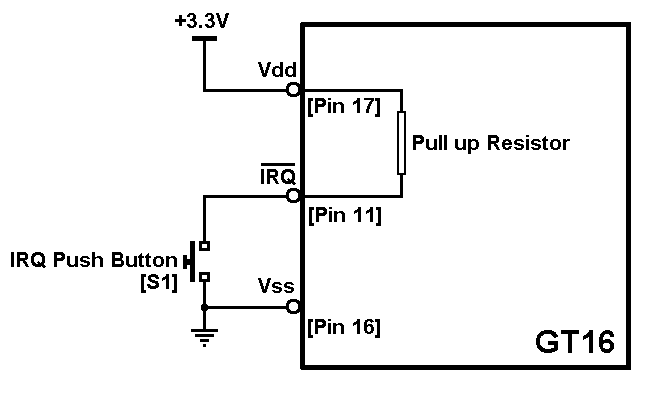
\includegraphics[width=0.7\textwidth]{figures/model.png}
% \caption{A block diagram illustrating the connections to the IRQ pin on the MCS08GT16A microcontroller (Please
% note that your headings should be short descriptions of what is in the diagram not simply the figure title)}
% \label{fig:model}
% \end{figure}

